\documentclass{article}
\usepackage[utf8]{inputenc}
\usepackage{xcolor}
\usepackage{graphicx}
\usepackage{hyperref}


\title{EPOCH and VisIt tutorial}
\author{FELICIA HOUNG TEEN TEEN}
\date{October 2022}


\begin{document}
\maketitle

\section{Prerequisite Packages}
\subsection{Fortran Compiler}
\begin{enumerate}
    \item First of all, to use EPOCH, you need fortran compiler. To find out if you have it, on the terminal, type \textcolor{red}{which gfortran}. If you have it installed, this \textcolor{red}{/usr/local/bin/gfortran} will be your output.
    \item To download gfortran, please follow the instructions here \url{https://gcc.gnu.org/wiki/GFortranBinaries}.
    \item You can choose to use Homebrew for the installation if you are using Mac.  \url{https://formulae.brew.sh/formula/gcc#default}
\end{enumerate}

\subsection{OpenMPI}
\begin{enumerate}
    \item Install OpenMPI by following the instructions here \url{https://formulae.brew.sh/formula/open-mpi}
    \item If you are downloading OpenMPI using another method, make sure you download the latest version for the EPOCH code to run.
\end{enumerate}

\subsection{CMake}
\begin{enumerate}
\item Download and install CMake \url{https://cmake.org/download/}
\item On terminal, add path \textcolor{red}{export PATH=$\$$PATH:$\$$HOME/Applications/CMake.app} into either one your system uses. For
\begin{enumerate}{}
    \item bash \\
    \textcolor{red}{nano $\sim$/.bash$\textunderscore$profile} or \textcolor{red}{nano $\sim$/.bashrc}
    \item zsh \\
    \textcolor{red}{nano $\sim$/.zsh$\textunderscore$profile} or \textcolor{red}{nano $\sim$/.zshrc}
\end{enumerate}
\end{enumerate}

\section{EPOCH}
\begin{enumerate}
    \item Compile EPOCH if it is your first time running it by changing to the correct working directory that you store your data. Taking 2D EPOCH as an example, switch to epoch2d by using this command \\
    \textcolor{red}{cd $\$$HOME/epoch/epoch2d} \\
    \item Type\\
    \textcolor{red}{make} or \textcolor{red}{make COMPILER=gfortran} (if the former doesn't work) to compile the code. A new directory called "bin" containing all the compiled binary naming \textcolor{red}{epoch1d}, \textcolor{red}{epoch2d}, \textcolor{red}{epoch3d} will be created after code compilation.\\
    \item Execute the binary file by typing \textcolor{red}{./bin/epoch2d} and the code will run. You shall see the EPOCH logo and things like this.

\begin{figure}[htp]
    \centering
    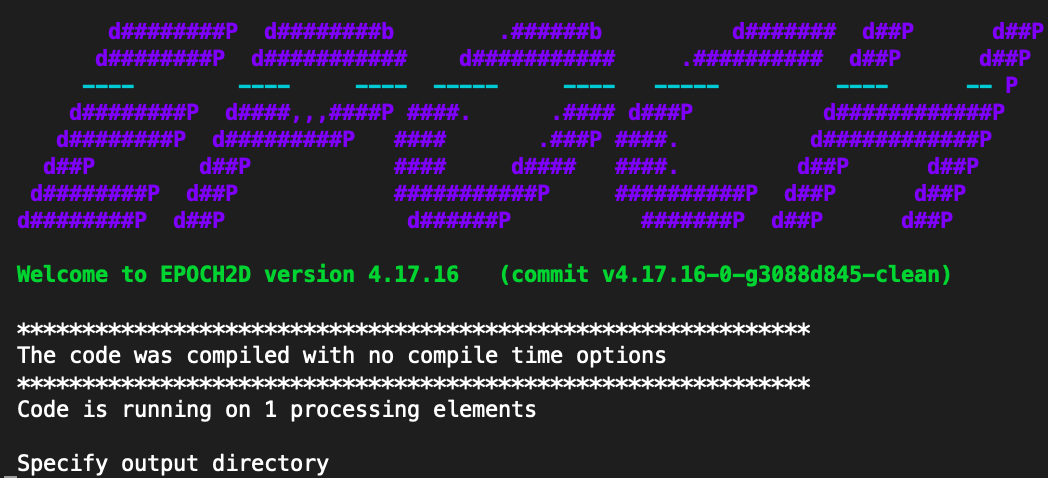
\includegraphics[scale=0.3]{EPOCH.png}
    \caption{EPOCH Logo}
\end{figure}

\item Type \textcolor{red}{./Data}, then the code shall run. Note that there must be a file name \textcolor{red}{input.deck} in the Data folder. Otherwise you have to copy the \textcolor{red}{deck} file you intend to run and paste it in \textcolor{red}{Data} folder and name it as \textcolor{red}{input.deck}. Then only you run the code. Note that the example deck file used in this manual is \textcolor{red}{laser$\_$focus.deck}.
\end{enumerate}

\section{VisIt}
\noindent VisIt is needed to read the sdf file.
\begin{enumerate}
    \item Install VisIt here \url{https://visit-dav.github.io/visit-website/releases-as-tables/#latest}
    \item You can either choose to add VisIt to your path so that you can open it by typing \textcolor{red}{visit} on the terminal or just simply click on the app. You shall see this on your screen.
    \begin{figure}[htp]
        \centering
        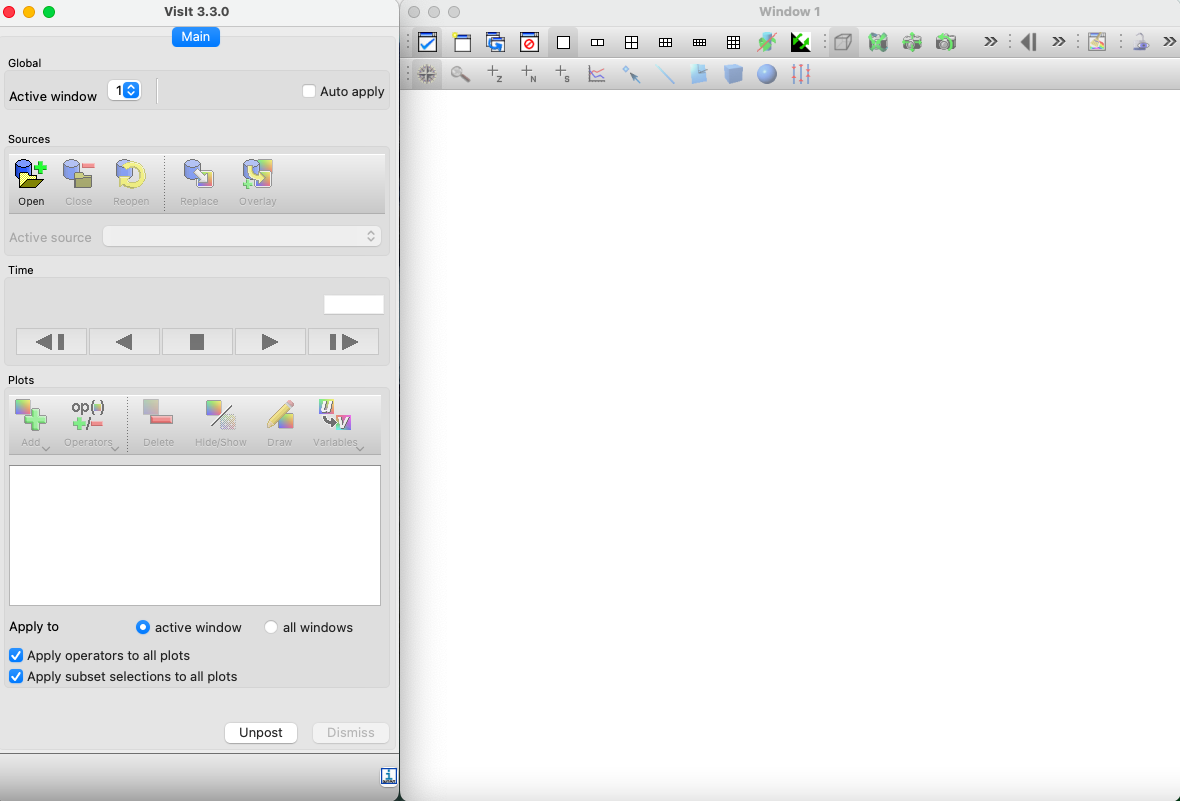
\includegraphics[scale=0.3]{VisIt.png}
        \caption{VisIt}
        \label{fig:my_label}
    \end{figure}
    \item Then, follow the procedure on the pictures.
    \begin{figure}[htp]
        \centering
        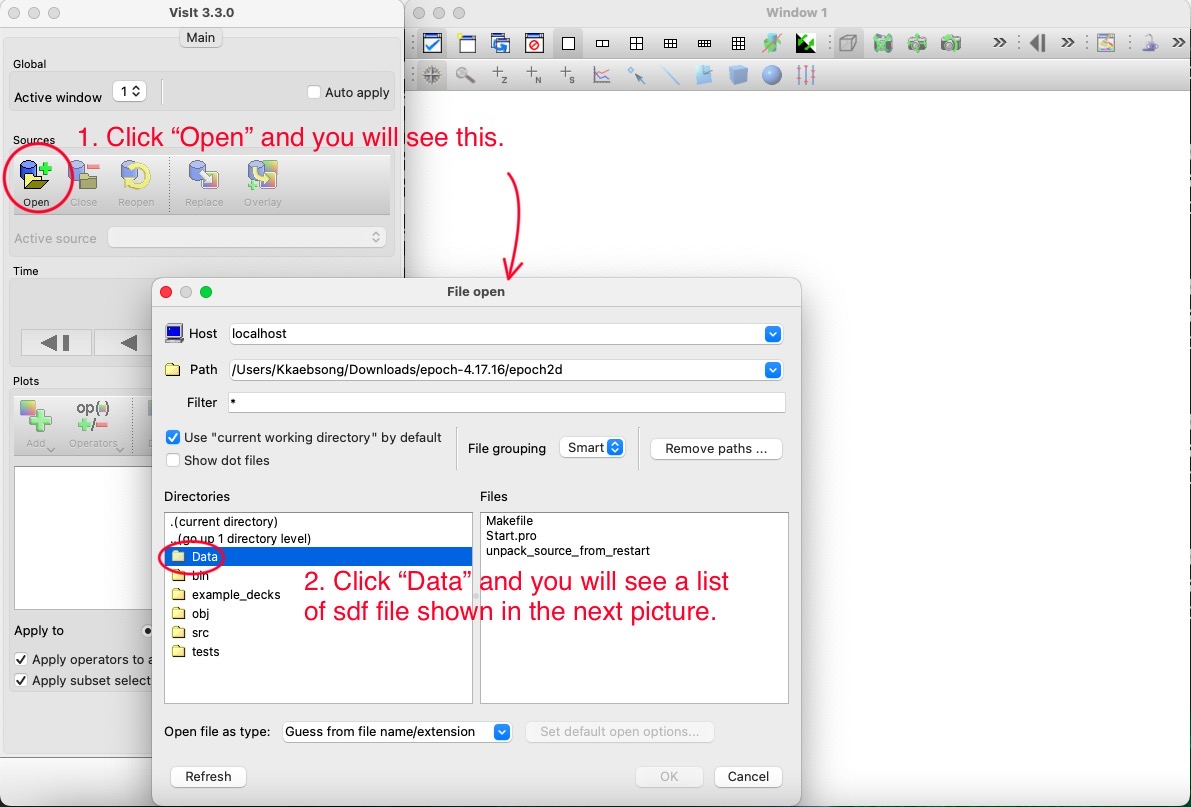
\includegraphics[scale=0.3]{VisIt2.jpg}
        \caption{VisIt}
        \label{fig:my_label}
    \end{figure}
    \begin{figure}[htp]
        \centering
        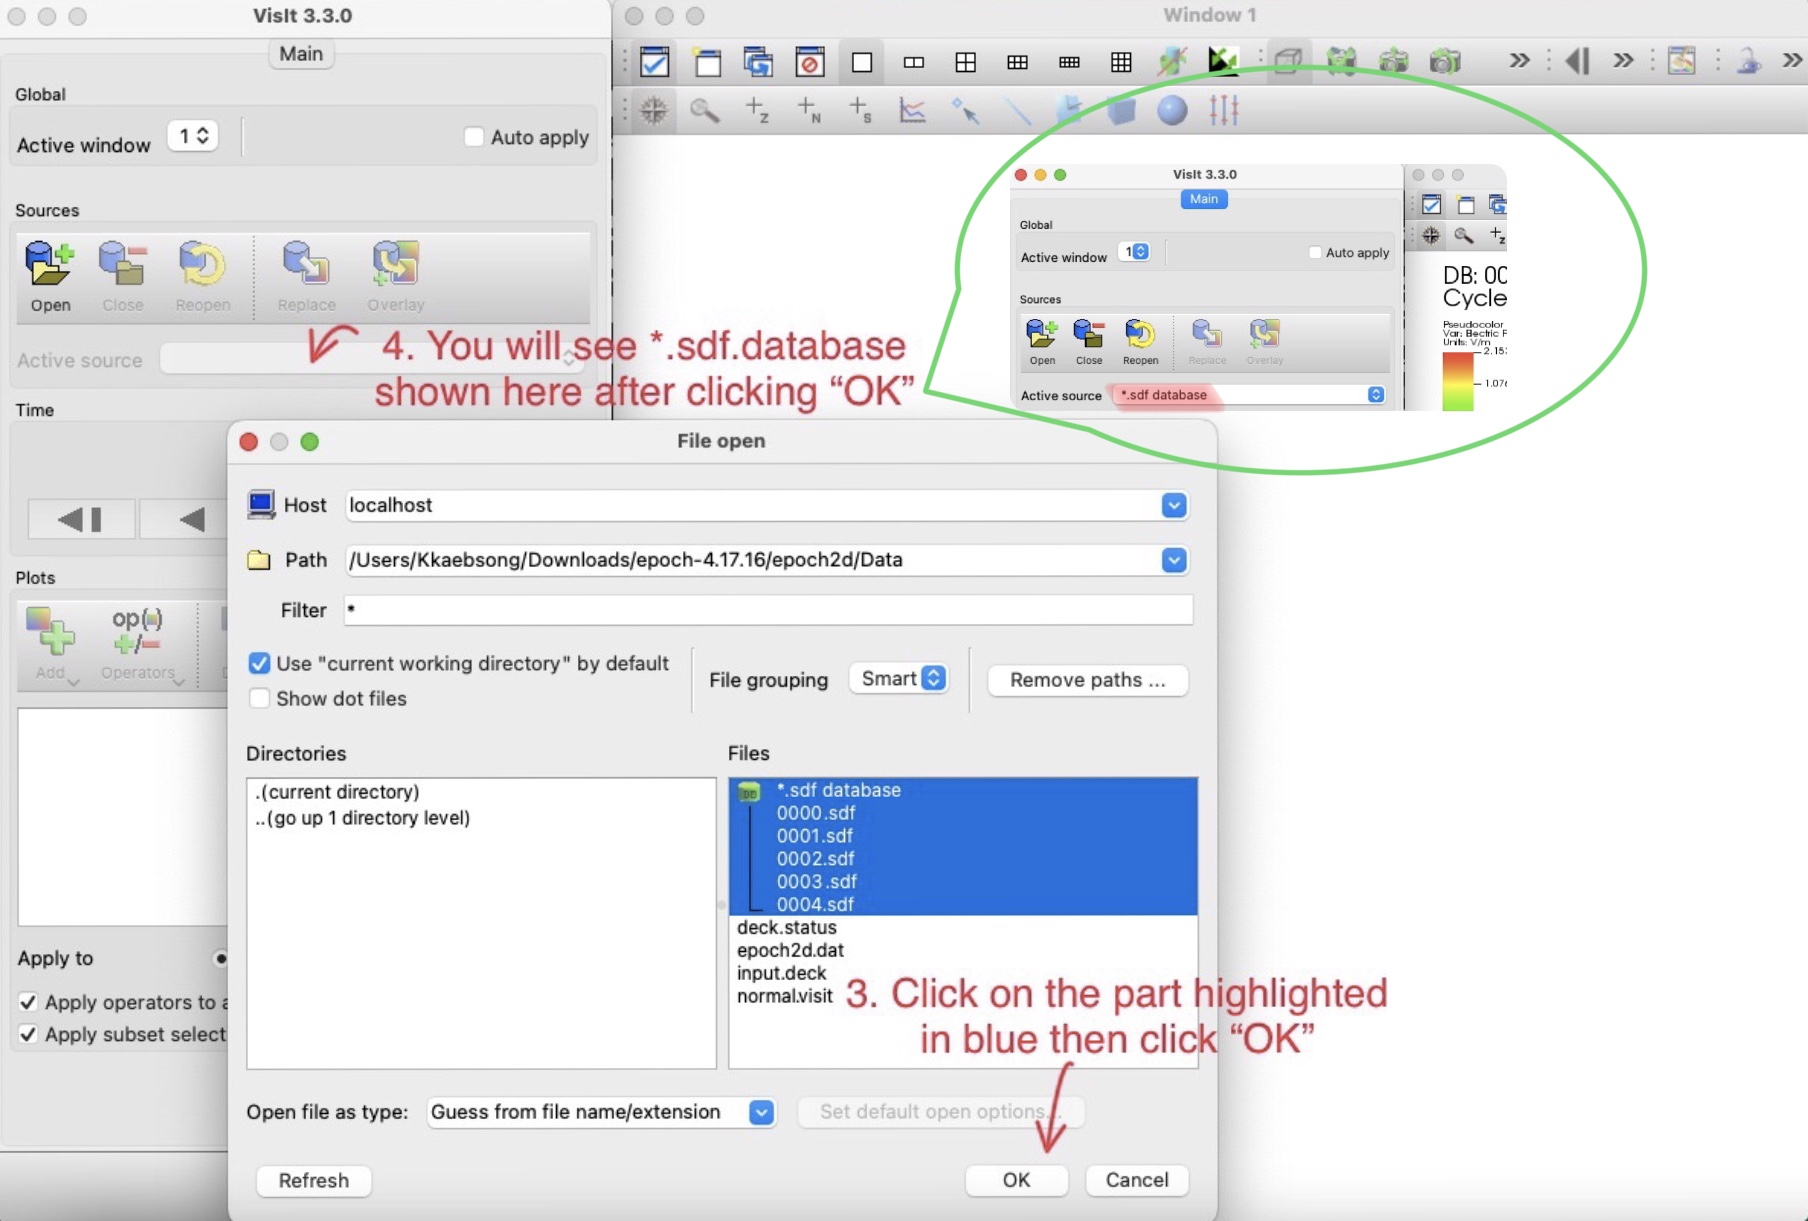
\includegraphics[scale=0.2]{Visit3.jpg}
        \caption{VisIt}
        \label{fig:my_label}
    \end{figure}
        \begin{figure}[htp]
        \centering
        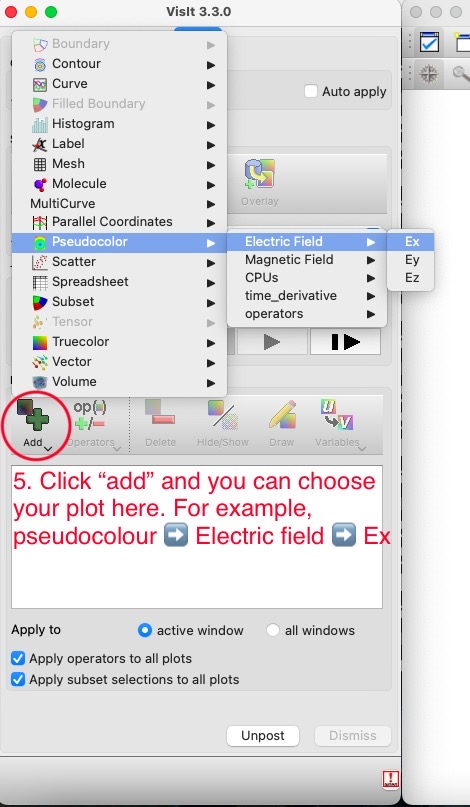
\includegraphics[scale=0.3]{visit4.jpg}
        \caption{VisIt}
        \label{fig:my_label}
    \end{figure}
        \begin{figure}[htp]
        \centering
        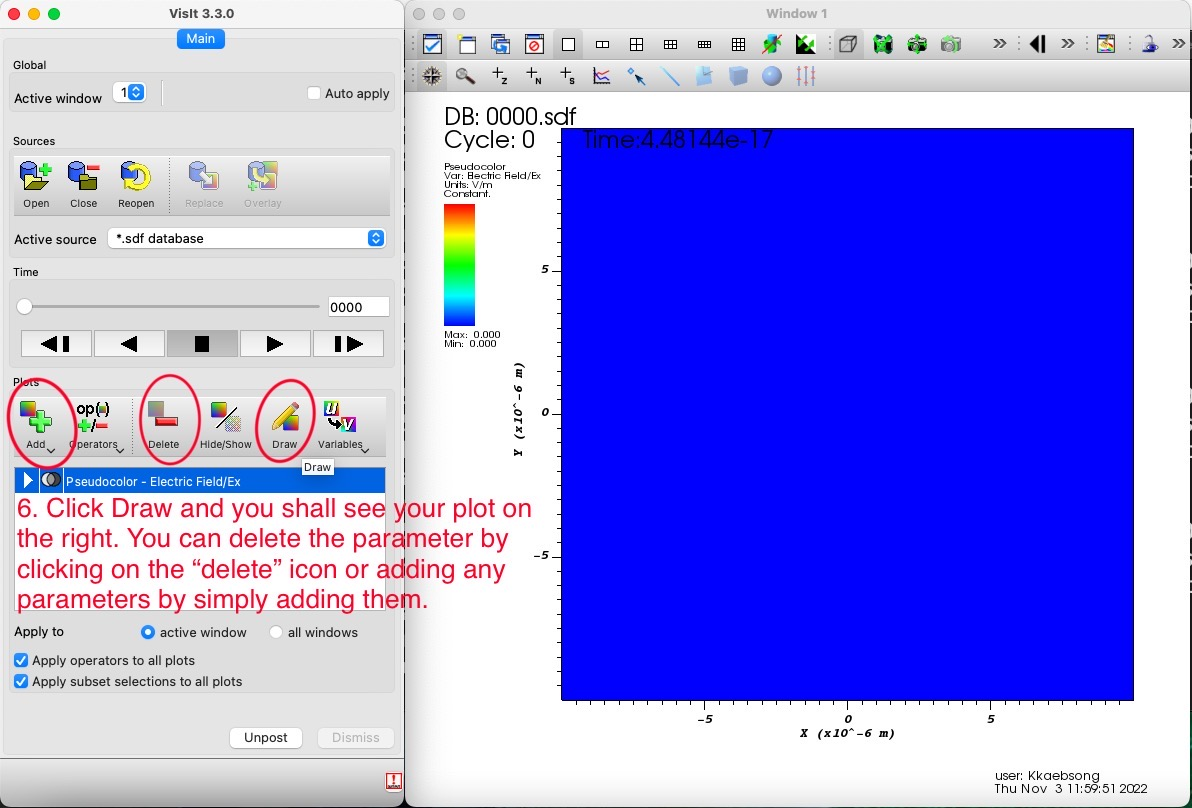
\includegraphics[scale=0.3]{visit5.jpg}
        \caption{VisIt}
        \label{fig:my_label}
    \end{figure}
        \begin{figure}[htp]
        \centering
        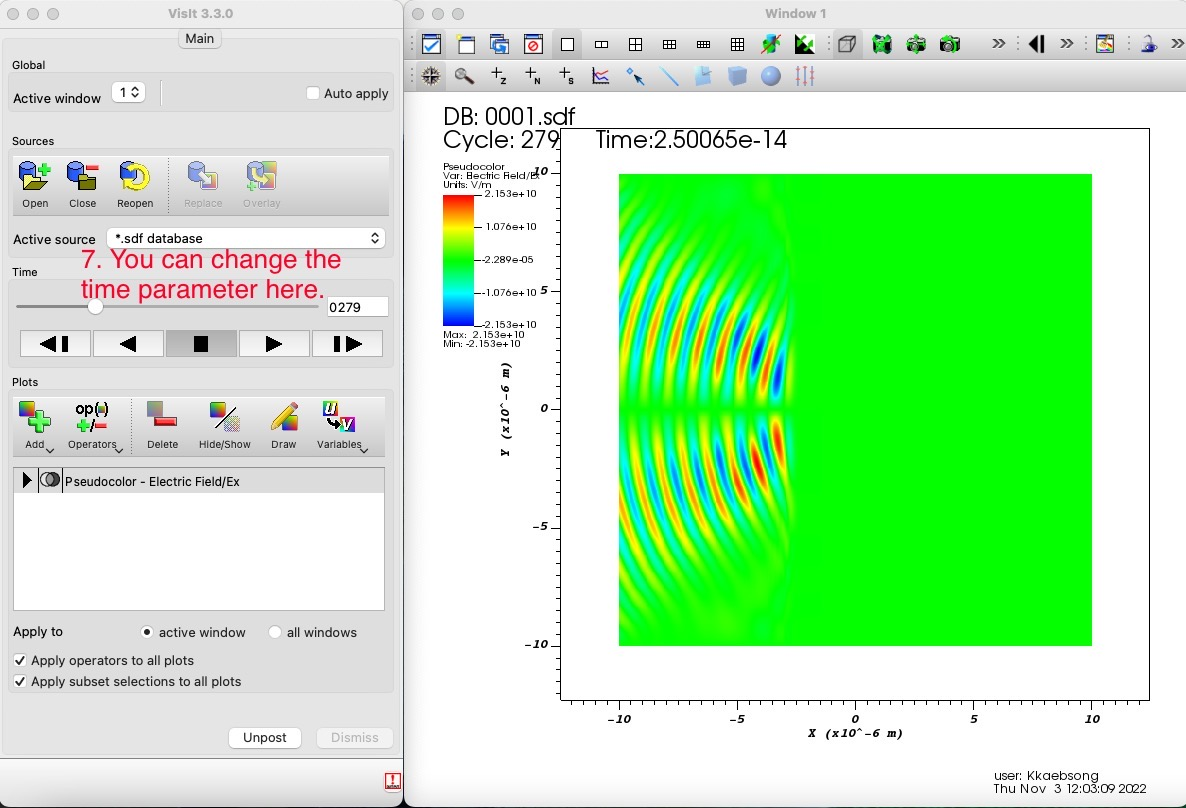
\includegraphics[scale=0.3]{visit6.jpg}
        \caption{VisIt}
        \label{fig:my_label}
    \end{figure}
\end{enumerate}


\end{document}
